\chapter{Background}
\onehalfspacing
\section{Speech signals}
Speech consists of a combination of sounds that form the human voice. The human voice propagates through air as localized vibrations that create small periodic fluctuations in air pressure. These vibrations enable the propagation of sound waves through the medium. The sound waves captured by microphones are converted into electrical signals, such as voltage or current variations. A speech signal can then be represented in a digital form in a view of waveform\cite{schroeder}.

\section{Waveform (Time Domain Representation)}
The waveform is the most straightforward representation of a speech signal, where the amplitude of the signal is plotted as a function of time. This view directly corresponds to how the signal is captured by a microphone and stored in digital form. In the time domain, important features such as speech energy, pauses, and major phonetic events can be observed. For example, the Figure \ref{fig:figure1} represents a male voice pronouncing a phrase - ”Illustration of typical speech signal waveform”.

\begin{figure}[htbp]
    \centering
    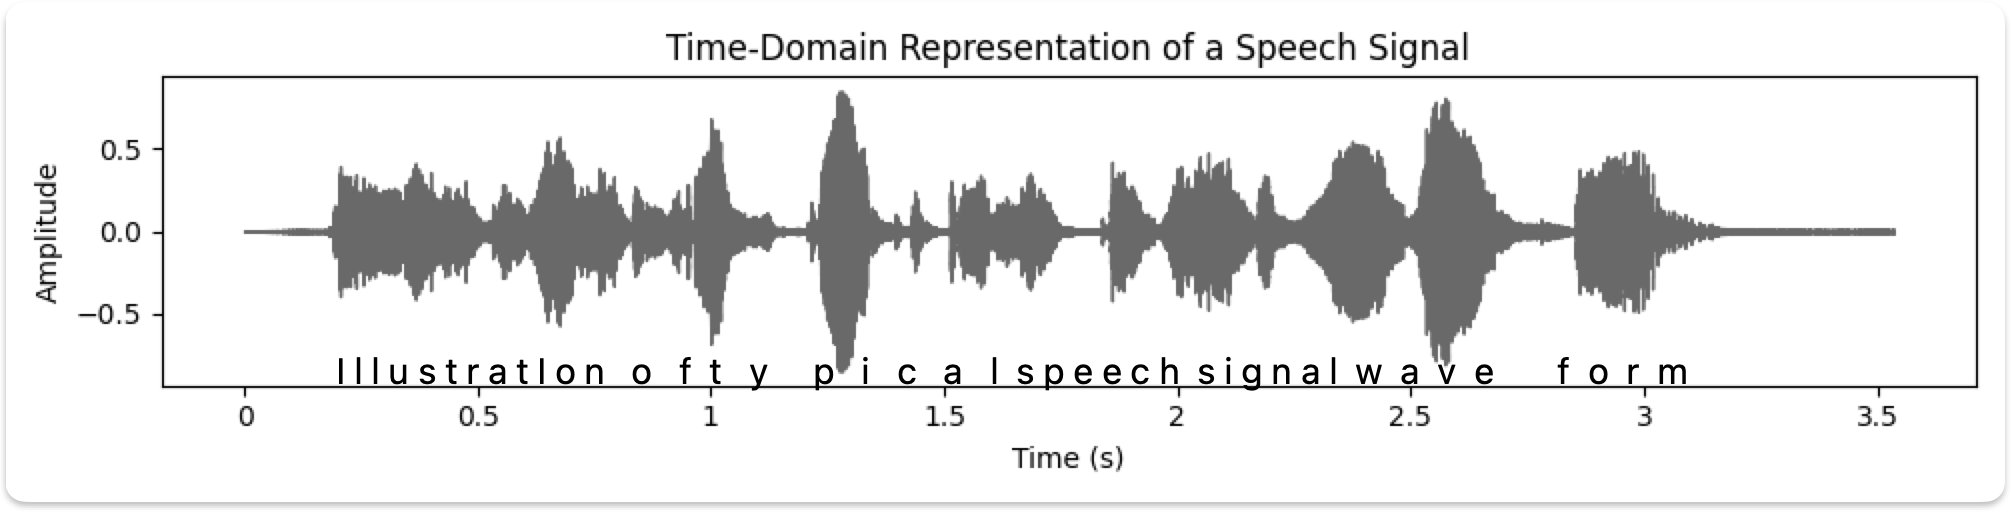
\includegraphics[width=.8\linewidth]{figures/figure7_waveform.jpg}
    \caption{Waveform of male voice.}
    \label{fig:figure1}
\end{figure}



\section{Fourier Transform (Frequency Domain Representation)}
While the time domain shows how the signal evolves over time, it does not reveal the frequency components that make up the signal.  
By applying the Fourier Transform (FT), the speech signal can be analyzed in the frequency domain, revealing which frequencies are present and their relative strengths.  
This is particularly important for understanding speech, as different sounds (such as vowels and consonants) occupy different frequency bands (Figure \ref{fig:figure2}). 


\begin{figure}[htbp]
    \centering
    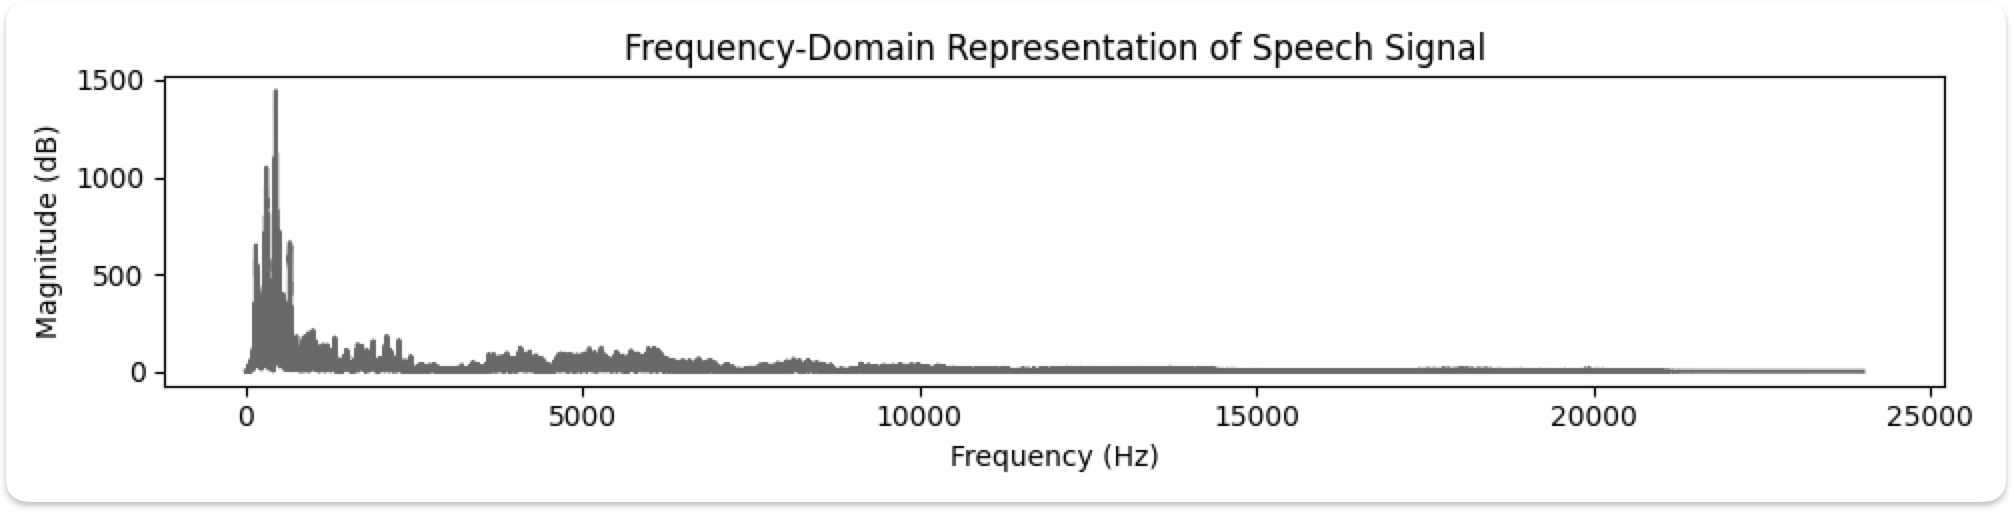
\includegraphics[width=.8\linewidth]{figures/figure8_1_fd.jpg}
    \caption{Speech Signal in a frequency domain.}
    \label{fig:figure2}
\end{figure}


\section{Spectrogram (Time–Frequency Representation)}

Speech signals are non-stationary, meaning their frequency content changes over time.
A spectrogram shows how the frequencies of a signal vary over time by applying the Short-Time Fourier Transform (STFT).

For machine learning applications, it is often better to use a Mel-Spectrogram (Figure \ref{fig:figure3}). Mel-Spectrograms are transformed spectrograms where frequencies are scaled to match how human ears perceive sound. After FT, it passes the result through a set of Mel filters that group frequencies in a way that matches how humans hear sounds.

Mel-Spectrograms represent the energy distribution of a speech signal across time and frequency and emphasize the perceptually important components of speech like formants (special frequencies that make each vowel sound different), harmonics (echoes of the main human voice pitch) and transitions between phonemes (single speech sounds, like "a", "s", "m") \cite{luitel2024audio}.


\begin{figure}[htbp]
    \centering
    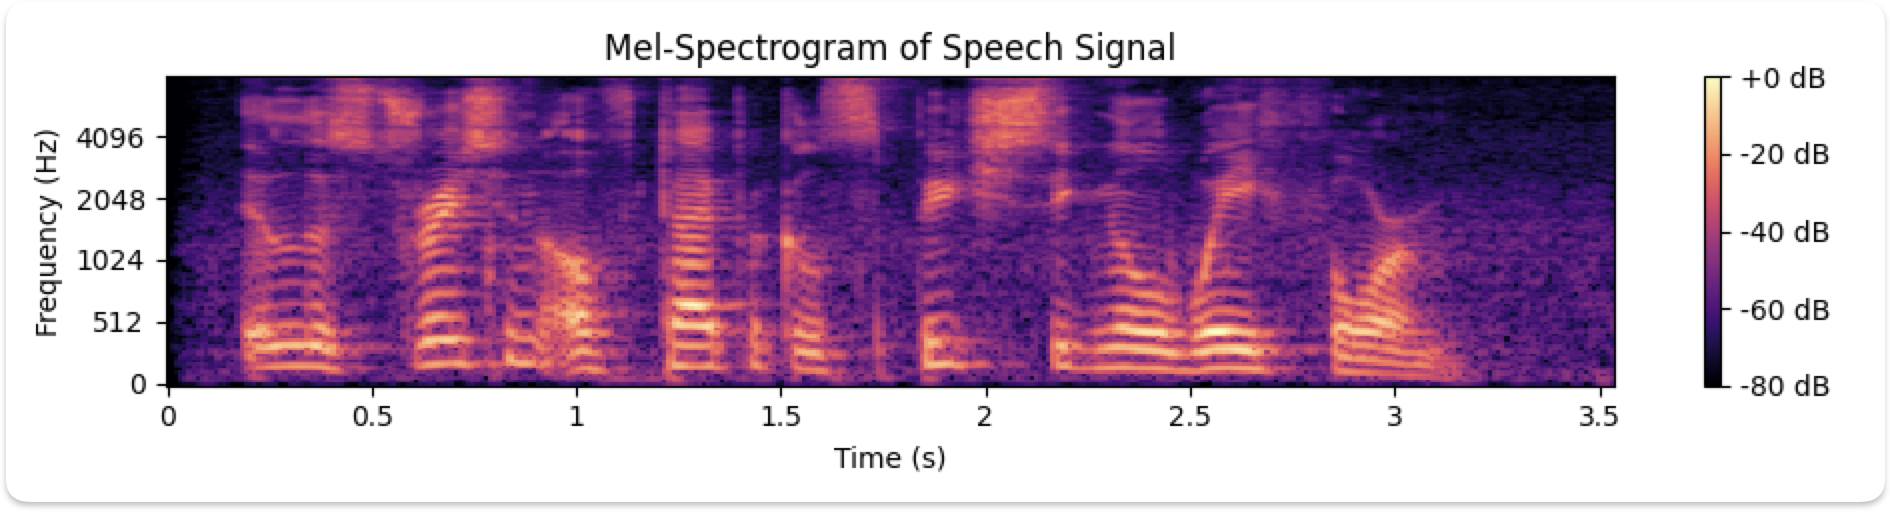
\includegraphics[width=.8\linewidth]{figures/mel-spectrogram.jpg}
    \caption{Mel-Spectrogram.}
    \label{fig:figure3}
\end{figure}


\section{The noise effect on speech signal}
As mentioned earlier, signal may be degraded or corrupted at various stages of speech signal processing. The illustration below clearly demonstrates how the signal from Figure \ref{fig:figure4} changes after the introduction of noise in the speech signal. The plot represents a continuous degradation of the signal.

\begin{figure}[htbp]
    \centering
    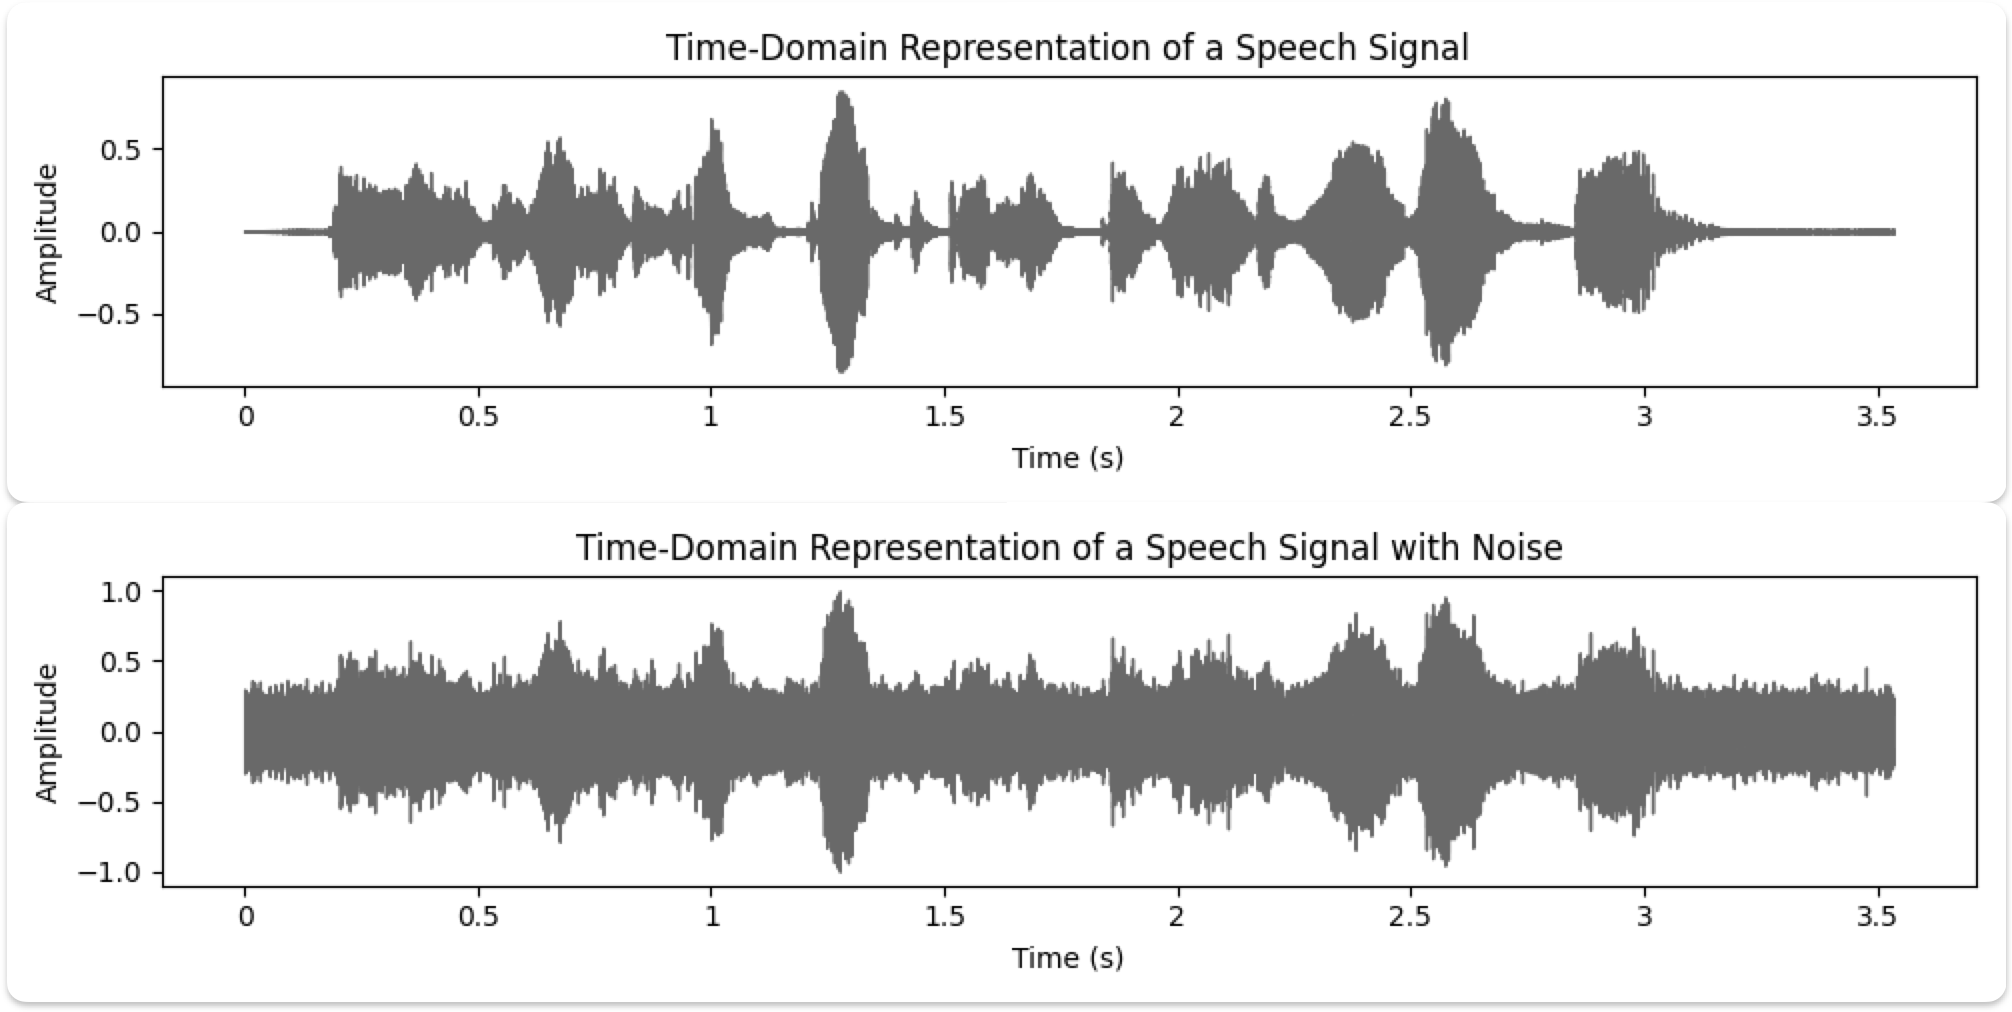
\includegraphics[width=0.8\linewidth]{figures/signal-with-a-gap.png}
     \caption{Waveform graphs of the original and noised signals.}
    \label{fig:figure4}
\end{figure}


The graph of the speech signal clearly shows changes compared to the original graph. 
 The lower waveform represents a case where the entire signal is covered by noise, masking the original speech content. When listening to the recording, the speech would sound distorted or buried under noise, making it difficult to perceive or understand. Such a signal disruption is unnatural and may occur due to environmental interference, low-quality recording conditions, or faulty equipment. Almost any part of the audio pipeline can contribute to this issue.
The loss of the audio signal can significantly reduce sound quality, making it a critical issue.


\section{Audio Inpainting}

Audio restoration refers to reconstructing degraded or corrupted parts of an audio signal. Just as image restoration removes noise and artifacts to recover visual quality, speech restoration aims to enhance clarity and naturalness in audio that has been affected by noise or distortion. In many real-world scenarios, the speech signal is not missing entirely but is masked by continuous or non-stationary background noise. Rather than identifying and filling silent gaps, the restoration process involves estimating a clean version of the speech signal from its noisy counterpart. Deep learning models, such as MetricGAN, enable this by learning perceptual representations of clean audio and optimizing the output to sound natural and intelligible, even when the original signal is heavily corrupted \cite{miotello}.


% \section{Deep Learning for Audio Inpainting}

% Deep learning refers to the field of training large neural networks with multiple layers to learn complex data patterns and has become a powerful tool for solving complex problems in signal processing, including the restoration of missing parts in audio signals \cite{ai-blog}.


% Deep learning has shown great potential for restoring missing parts of audio signals. One example is the work by Marafioti et al.~\cite{marafioti}, who proposed a context encoder that learns from the surrounding time–frequency information of the Short-Time Fourier Transform (STFT) to predict missing segments. Their results showed that deep neural networks can outperform traditional methods in preserving the naturalness and continuity of audio.

% Another approach was proposed by Miotello et al.~\cite{miotello}, who used a deep prior technique, where the structure of a multi-resolution convolutional network helps guide the inpainting process. Their model was able to reconstruct missing audio fragments with high accuracy, even without needing large training datasets. 

% Both studies show the effectiveness of deep learning in solving the challenges of audio reconstruction.

\chapter{Speech Signal Enhancement Methods: MetricGAN and Wiener Filter}
A Generative Adversarial Network (GAN) consists of two parts:

The \textbf{generator} learns to generate realistic data. The generated samples serve as negative training examples for the discriminator.

The \textbf{discriminator} learns to distinguish the generator's fake data from real data. It penalizes the generator for producing unrealistic results.

At the beginning of training, the generator produces fake data, and the discriminator quickly learns to identify it as fake.
As training progresses, the generator improves and starts producing outputs that can fool the discriminator.
Eventually, if the generator trains well, the discriminator becomes less effective at distinguishing real from fake. It begins classifying fake data as real, and its accuracy decreases.

Both the generator and the discriminator are neural networks. The generator's output is directly connected to the discriminator's input. Through backpropagation, the discriminator's classification provides a signal that the generator uses to update its weights \cite{metricgan}.

\section{MetricGAN Architecture for Audio Inpainting}

MetricGAN is a generative adversarial network model specifically designed for speech enhancement and restoration tasks. Unlike traditional models that optimize for signal similarity or statistical loss functions, MetricGAN is trained to directly optimize perceptual quality metrics (e.g., PESQ, STOI) by mimicking human perception of audio quality. This makes it well suited for enhancing noisy speech, even if the signal is entirely covered by background noise.

In speech tasks, the input to MetricGAN is a spectrogram of the noisy audio, and the output is a cleaned (enhanced) version of the spectrogram. Figure \ref{fig:figure5} illustrates this architecture: the generator takes in a magnitude spectrogram of the noisy signal and produces an enhanced spectrogram. The discriminator then compares the enhanced output against clean reference samples and estimates how close the perceptual quality is.

\begin{figure}[htbp]
    \centering
    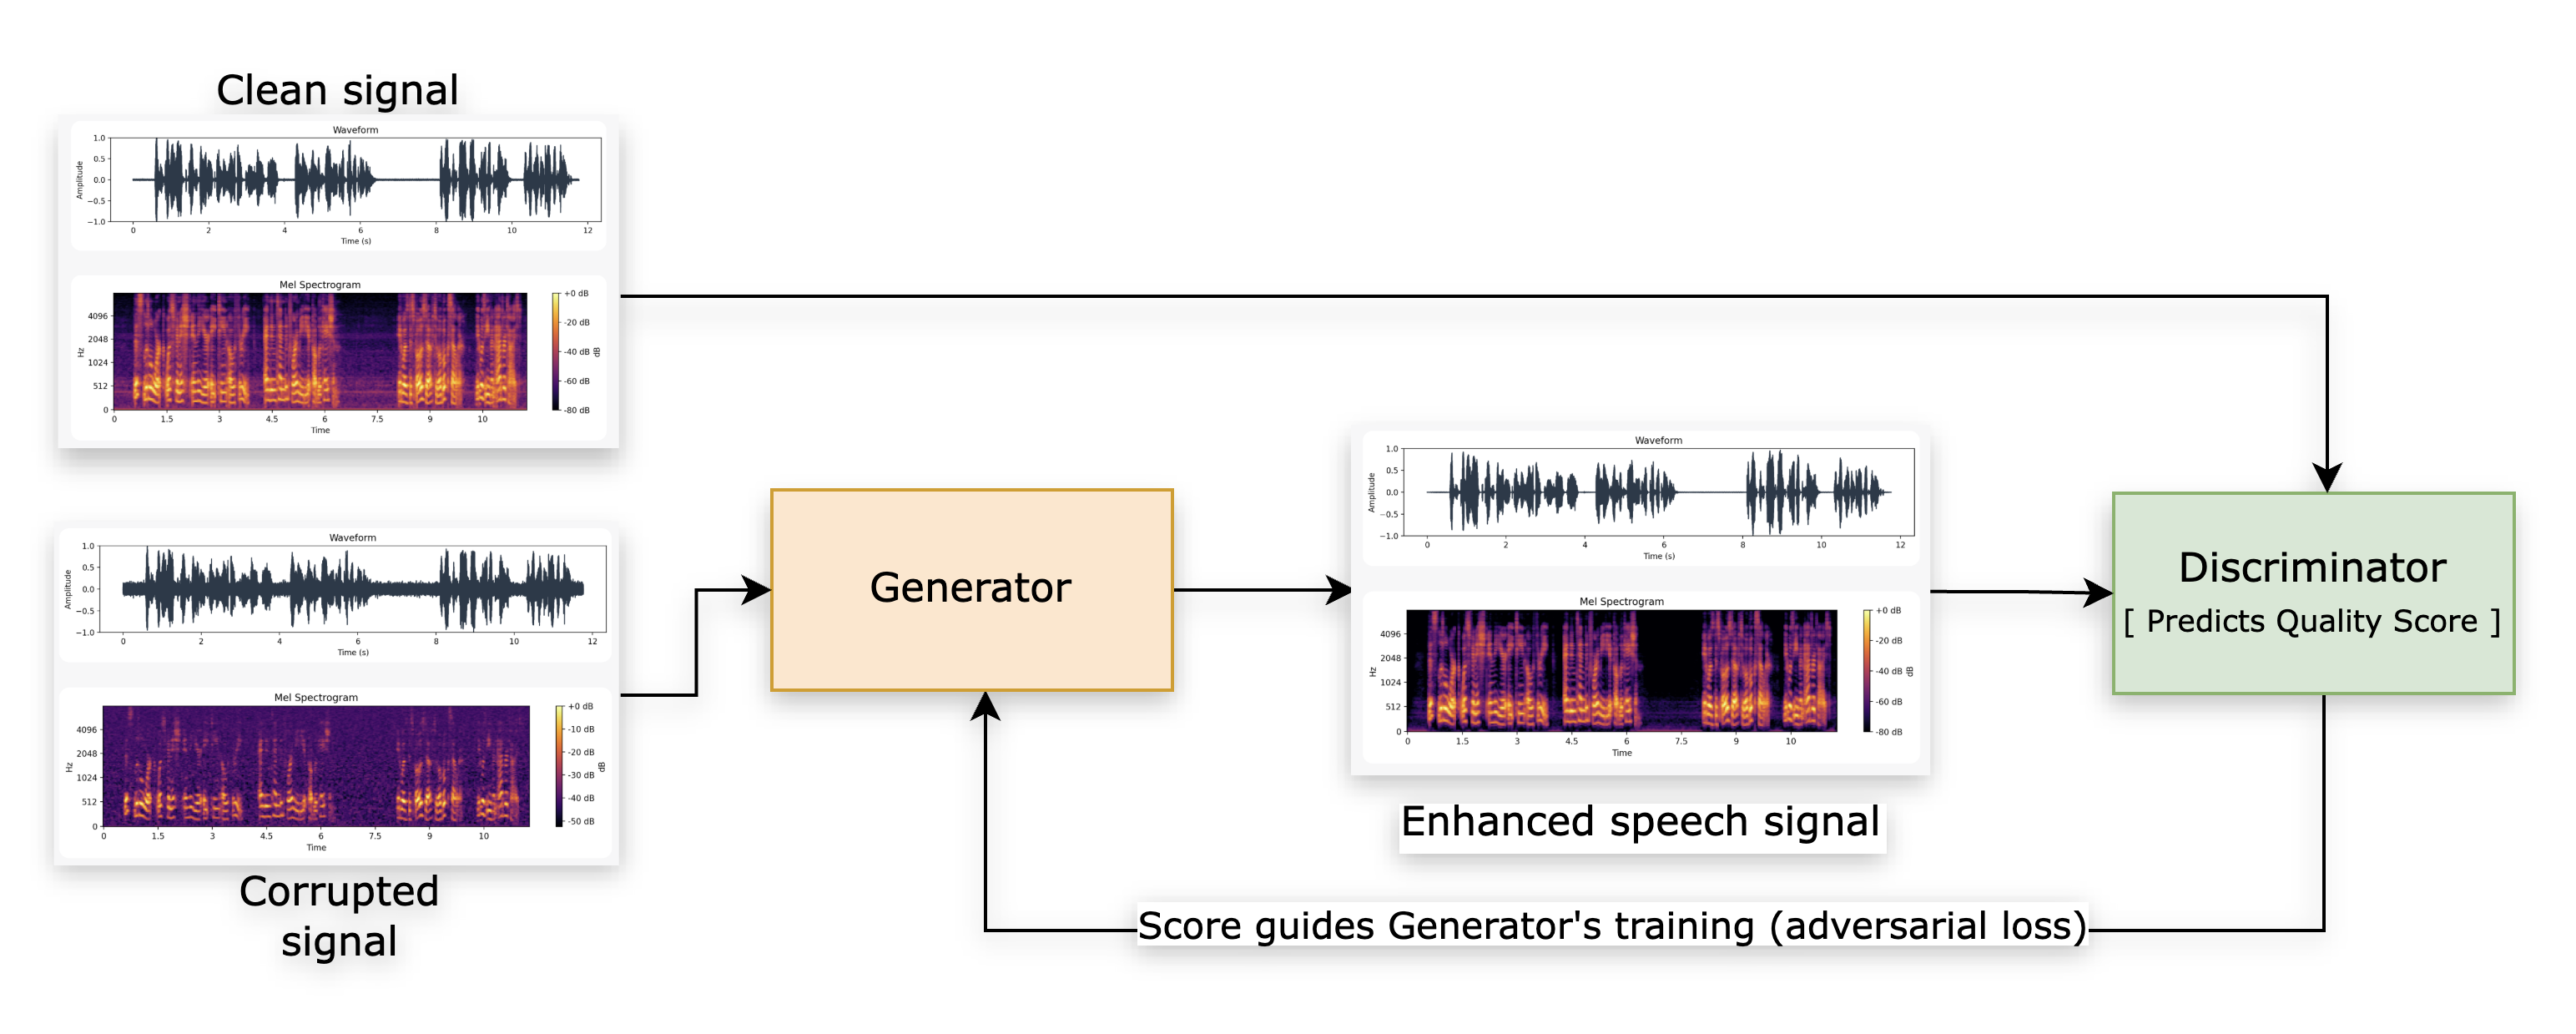
\includegraphics[width=1\linewidth]{figures/MetricGAN.png}
     \caption{High Level MetricGAN architecture. The generator produces enhanced audio, while the discriminator evaluates perceptual quality.}
    \label{fig:figure5}
\end{figure}

In a typical GAN structure, two neural networks - a generator and a discriminator — are trained in opposition. The generator learns to map a noisy audio input to its clean counterpart, while the discriminator evaluates how perceptually close the generated output is to a real, clean audio signal. What sets MetricGAN apart is that the discriminator is trained not just to classify real vs. fake, but to predict quality scores based on objective intelligibility and perceptual metrics.

Figure \ref{fig:figure6} illustrates the training process of the MetricGAN architecture, where the generator progressively enhances noisy speech signals. Over time, the quality of the enhanced output improves, as indicated by increasing PESQ scores: low (\(<\) 2.0), intermediate (2.0- 4.0), and high (\(>\) 4.0).

The generator produces enhanced audio from a corrupted input. This output is then evaluated by the discriminator, which predicts a perceptual quality score (PESQ) by comparing the enhanced signal to the clean reference. The predicted score is used to update the generator's parameters via adversarial loss, encouraging it to produce outputs that are perceptually closer to clean speech.

The discriminator plays a key role in guiding the generator’s learning, not by classifying real vs. fake, but by providing a continuous score that reflects human-perceived quality.


MetricGAN is widely used in modern speech enhancement benchmarks and has demonstrated strong performance in restoring intelligibility and perceptual quality, especially in real-world noisy environments where traditional gap-filling methods are ineffective. Its ability to learn perceptual optimization rather than just signal-level accuracy makes it especially effective for continuous signal degradation tasks.


\begin{figure}[H]
    \centering
    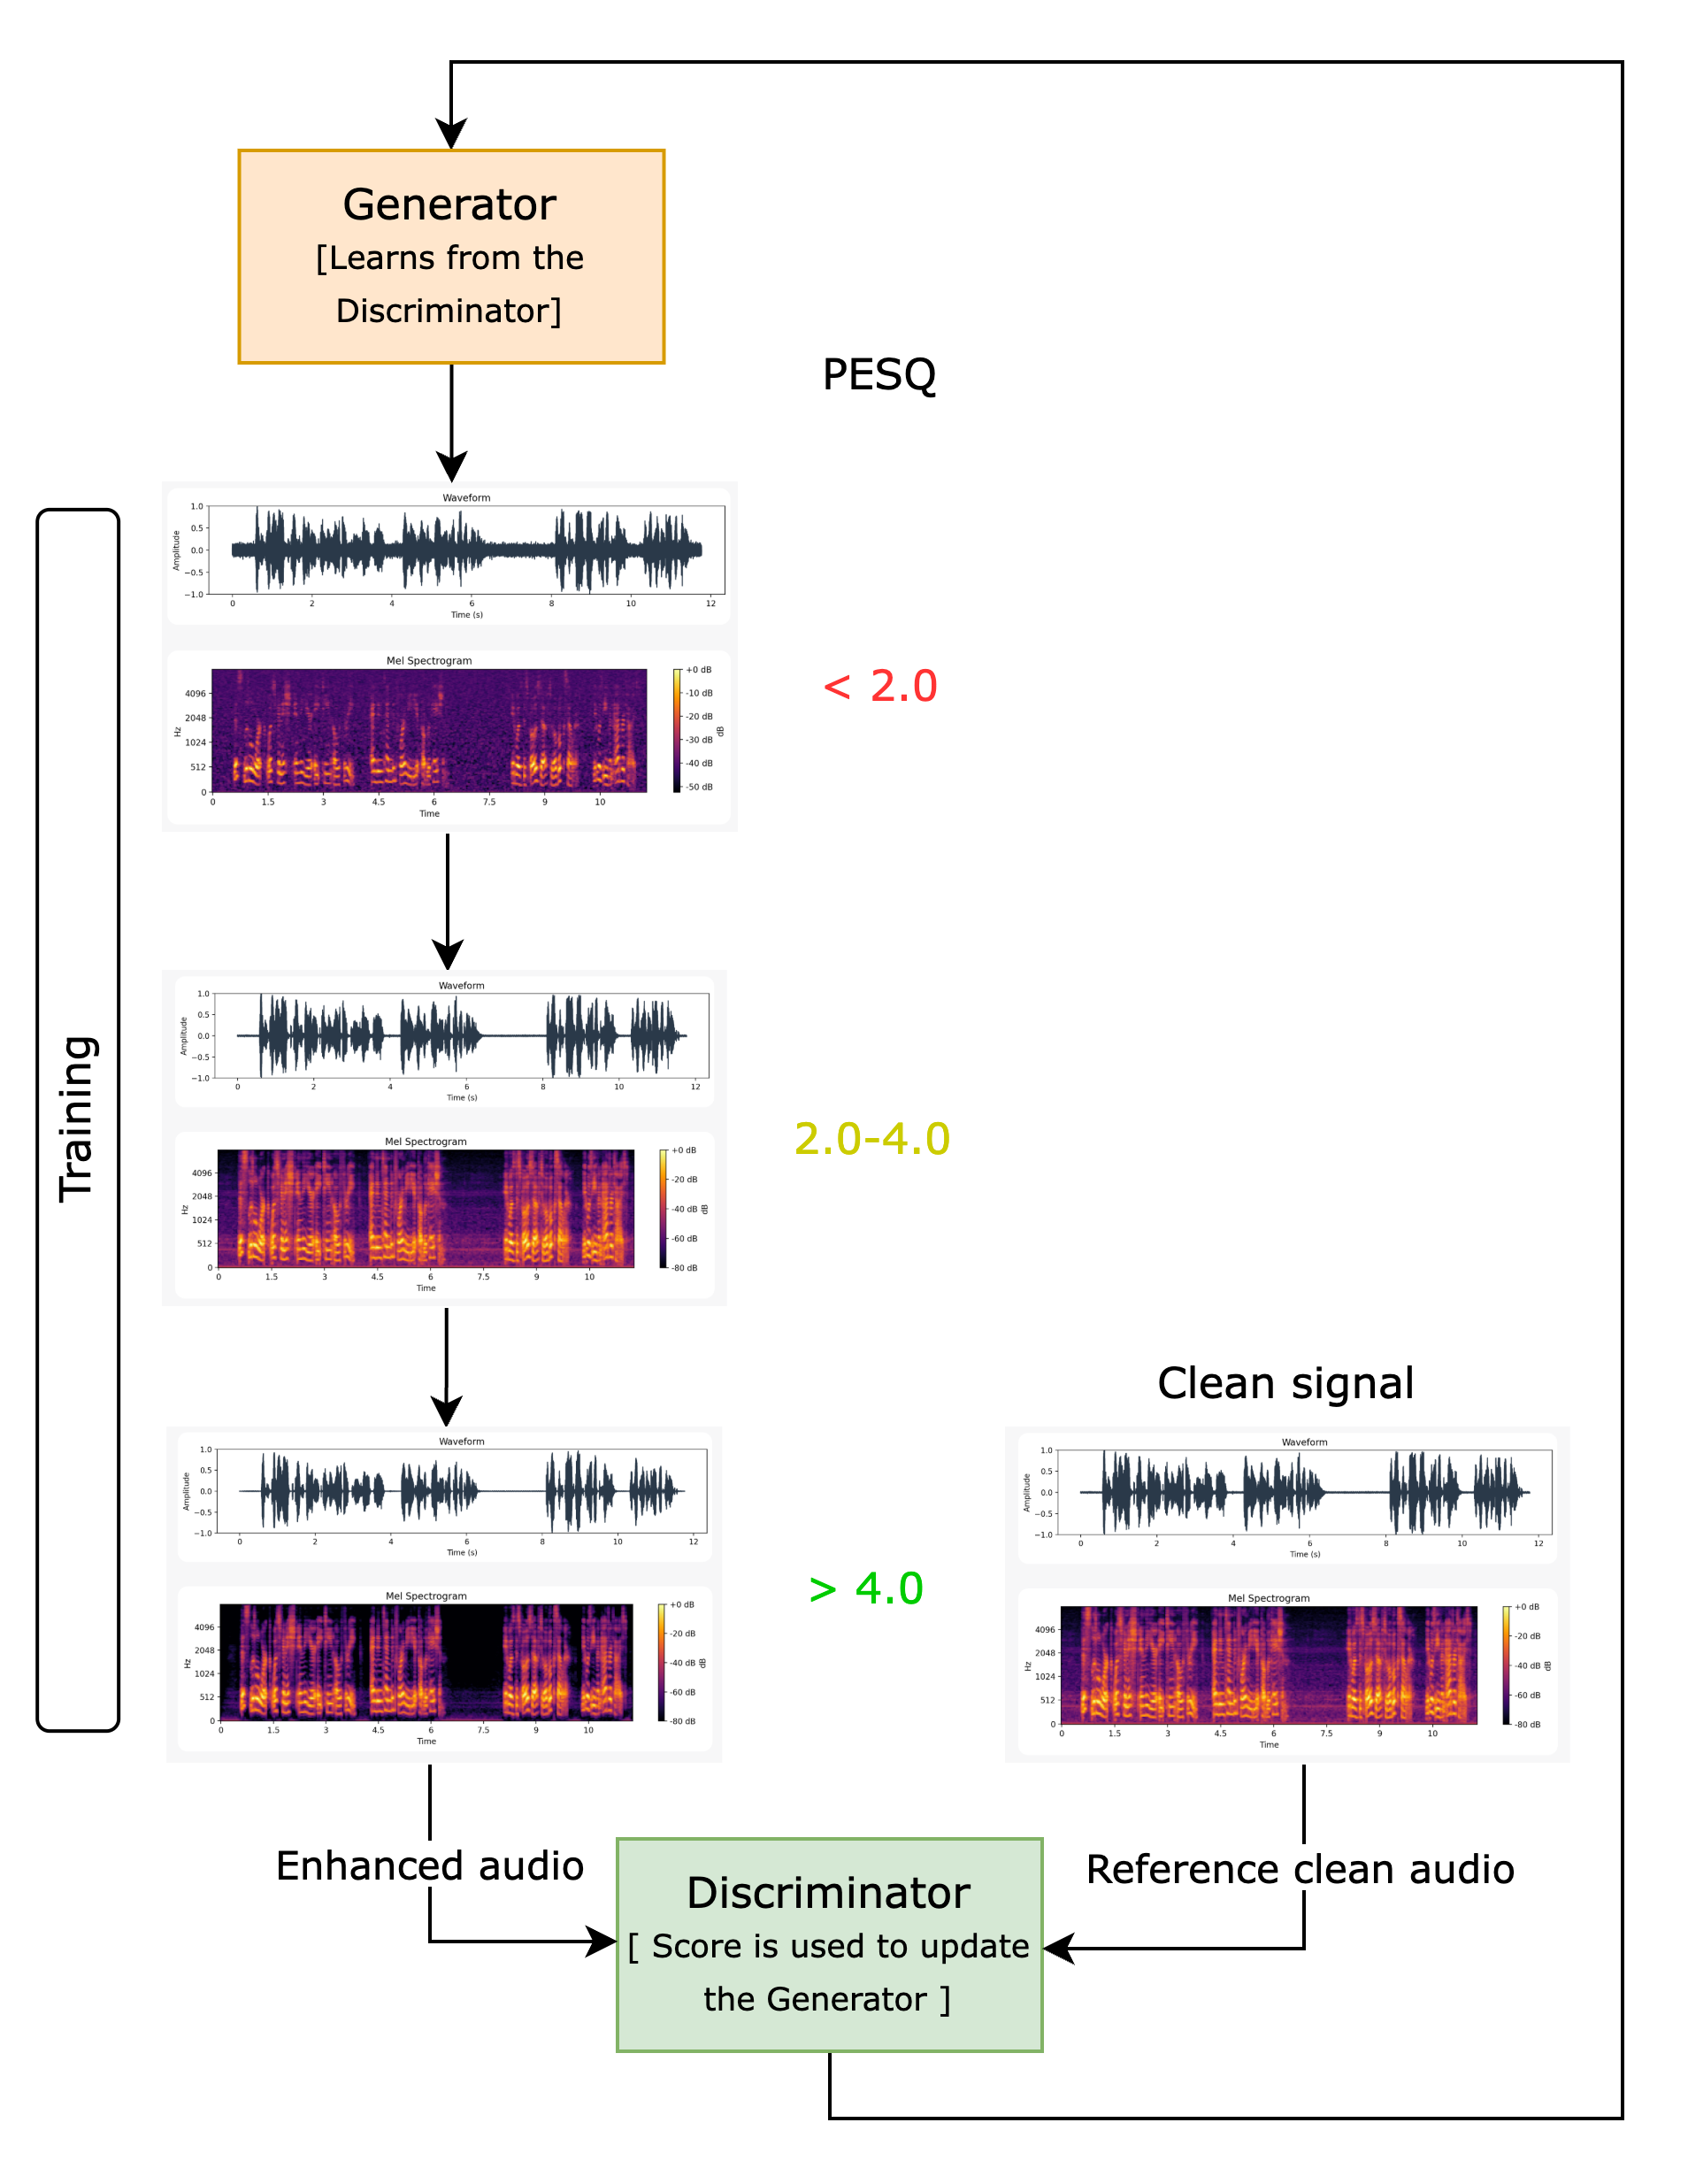
\includegraphics[width=.6\linewidth]{figures/gendis.png}
     \caption{MetricGAN Training Process Guided by PESQ Scores}
    \label{fig:figure6}
\end{figure}

\section{Wiener Filter for Speech Enhancement}

One of the classical approaches to speech signal reconstruction is Wiener filtering. Originally developed by Norbert Wiener, this method provides an optimal linear estimator of a clean signal from a noisy observation by minimizing the mean squared error (MSE).


In speech signal applications Wiener filtering is used to suppress noise and recover the clean speech. However, when noise is added, the clean and noisy components become dependent. As a result, the Wiener filter output contains both signals—typically with speech as the dominant component and noise as a residual minor part.

The Wiener filter works well when the noise level can be estimated accurately, usually during moments of silence in the recording. Its performance becomes worse when the missing parts are long or when the background noise changes over time. \cite{reddy}


Due to its historical importance and solid theoretical foundation, Wiener filtering has often been a baseline method in speech enhancement and restoration tasks. A detailed discussion of its application in speech processing can be found in the textbook by Loizou~\cite{loizou}, which remains one of the standard references in the field.

\chapter{Evaluation Metrics}

To objectively assess the quality of reconstructed speech signals, several evaluation metrics are commonly used. In this work, the reconstruction performance is measured using SNR, PESQ, and STOI.

\section{Perceptual Evaluation of Speech Quality}
PESQ - is an objective method used to assess the quality of speech signals after transmission or compression. It was developed to improve upon earlier models by accurately predicting perceived speech quality across a wide range of network conditions, including codec distortions, packet loss, filtering, and variable delays.

PESQ operates by comparing a reference (clean) speech signal with a degraded version. The perceived distortions are then calculated by analyzing the difference in loudness across time and frequency. These distortions are aggregated using a non-linear method known as the \(L_p\) norm:

\[L_p = (\sum_{m=1}^{M}disturbance[m]^p)^{1/p}\]
where \(m\) indexes the time-frequency cells.

The final step predicts the Mean Opinion Score (MOS), which represents the subjective quality of the speech, using a simple linear formula:

\[PESQMOS = 4.5 - 0.1 \times d_{sym} - 0.0309 \times d_{asym}\]
where \(d_{sym}\) and \(d_{asym}\) are asymetric disturbance parameters.

PESQ ranges from 1.0 (bad quality) to 4.5 (excellent quality). Higher values indicate better speech quality closer to natural, undistorted speech. \cite{pesq}

PESQ is an essential metric in this thesis because it provides an objective way to evaluate the quality of reconstructed speech signals. By comparing the restored speech to the original, PESQ helps determine whether the reconstruction methods preserve the naturalness and intelligibility of the speech as perceived by human listeners.


\section{Short-Time Objective Intelligibility}
STOI measure is an objective method designed to predict the intelligibility of speech signals, especially after noise reduction or time-frequency processing. Unlike traditional measures that focus on long-term signal statistics, STOI operates on short-time regions (approximately 400 ms) to capture local degradations in speech.

STOI is based on comparing the clean speech signal \(x\) and the processed (degraded) speech signal \(y\). Both signals are divided into overlapping short frames, transformed into the frequency domain using a STFT, and grouped into one-third octave bands. Within each short-time region, STOI computes a local normalized correlation between the clean and processed signals:


\[d_j(m) = corr(X_j(n), Y'_j(n))\]
where \(X_j(n)\) and \(Y'_j(n)\) are energy representation of the clean and processed signals for a specific frequency band and time frame, and \(Y'_j(n)\) includes normalization and clipping to stabilize distortions. 

The final STOI score \(d\) is obtained by averaging these local correlations over all time frames and frequency bands:


\[d = \frac{1}{JM}\sum_{j,m}d_j(m)\]
where \(J\) is the number of frequency bands and \(M\) is the number of time frames.

STOI scores range from 0 to 1, where 1 indicates perfect intelligibility and 0 indicates completely unintelligible speech. \cite{stoi}

STOI provides an objective way to measure how understandable the reconstructed speech signals are. Since this thesis focuses on restoring missing parts of speech, STOI helps evaluate whether the reconstruction preserves the original speech intelligibility. A higher STOI score after reconstruction indicates better performance of the proposed methods.



\section{Signal-to-Noise Ratio}

SNR - is a measure that compares the level of the desired signal to the level of background noise. It tells how much stronger the useful signal is compared to the unwanted noise. A higher SNR indicates that the reconstructed signal is closer to the original, with less distortion.

Mathematically, SNR is the ratio of signal power \(S\) to noise power \(N\), and is usually expressed in decibels (dB) using the formula:

\[SNR(dB) = 10\log_{10}{(\frac{S}{N})}\]

When signal and noise powers are given in dBm, SNR can be calculated by subtracting the noise level from the signal level. A higher SNR means better signal quality and less interference:
\[SNR(dB) = Signal(dBm) - Noise(dBm)\]

SNR scores range typically from low negative values (e.g., -10 – 30 dB). Higher SDR indicates that less distortion is present in the reconstructed signal compared to the original. \cite{snr}

In the context of this thesis, SNR is used as an objective metric to evaluate the quality of reconstructed speech signals. A higher SNR after reconstruction indicates a more accurate and effective restoration of the missing components.